% Activate the following line by filling in the right side. If for example the name of the root file is Main.tex, write
% "...root = Main.tex" if the chapter file is in the same directory, and "...root = ../Main.tex" if the chapter is in a subdirectory.
 
%!TEX root =  ../Thesis.tex

\chapter[ATLASDetector]{Full Title}




\section{Introduction}

%http://home.web.cern.ch/about/accelerators
\section{CERN and the Large Hadron Collider}
The European Center for Nuclear Research (CERN) is a scientific complex in Geneva, Switzerland that was established in the years following World War II.  Its focus is experimental particle physics, in particular the Large Hadron Collider (LHC), although it also houses a theoretical physics department and numerous other experiments relating to the fundamental particles and their interactions.  

The LHC is the accelerator that serves as the centerpiece of CERN's scientific program.  The accelerator is circular and located in an underground tunnel with a circumference of 27 km, and when it is running, accelerates and collides two proton beams (sometimes two lead ion beams) at four points around the accelerator ring.  At each of these collision points is a detector designed to measure the particles resulting from the collisions: CMS, LHCb, ALICE, and the experiment where the data for this thesis was collected, ATLAS.

The LHC is the last and most powerful in a series of staged accelerator complexes, which in combination accelerate protons from rest to an energy of 4 TeV as of 2012.  Since there are 2 beams that collide head-on, the total center-of-mass energy is 8 TeV.  The first step in the process is the proton source, where hydrogen atoms are subjected to an electric field that separates the protons from the electrons.  Then the protons are accelerated by a 90kV field and focused, then sent to the linear collider.  From this point forward, all the accelerators use radio frequency (RF) electromagnetic waves to impart energy to the protons.  

The linear accelerator brings the protons up to an energy of 50 MeV, then they go to the Proton Synchrotron Booster (up to 1.4 GeV), and then the Proton Sychrotron (25 GeV).  Then the protons are passed to the Super Proton Synchrotron, where they reach an energy of 450 GeV, and finally the beam is split into half and each half is injected into the LHC going a different direction.  Figure ~\ref{fig:accelerator_complex} shows all the major accelerators at the CERN site.

%%% CERN accelerator figure
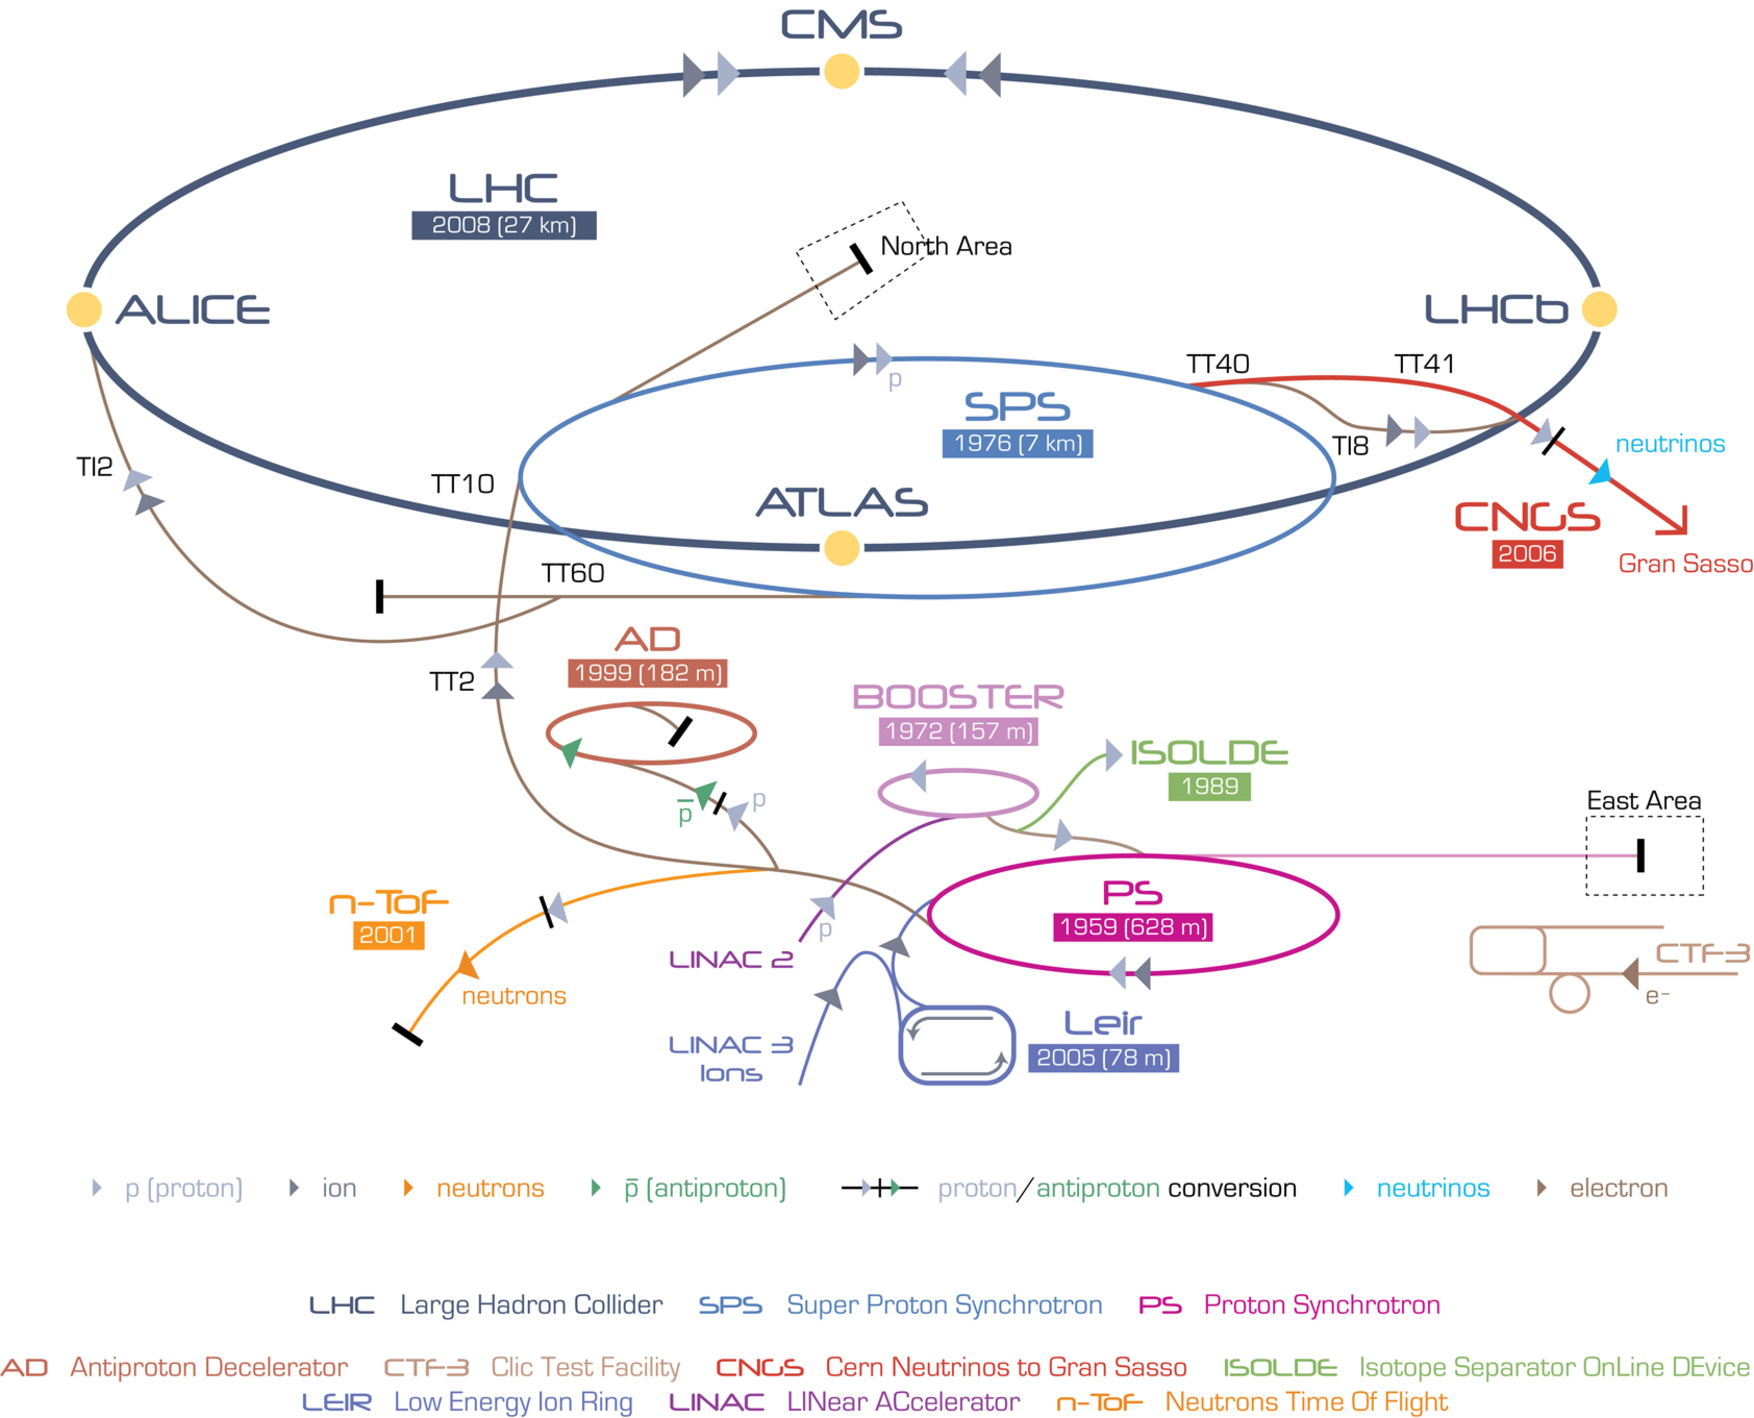
\includegraphics[width=\textwidth]{/Users/caitlinmalone/Documents/Thesis/ATLASDetector/images/Cern-Accelerator-Complex.pdf}\label{fig:accelerator_complex}

Once the beams are in the LHC, they are accelerated over the course of about 20 minutes up to the full collision energy of 4 TeV per beam.  Then the beams are focused at each of the 4 interaction points, and carefully steered into position so that head-on collisions commence.  The protons are arranged in bunches within the beams, with each bunch 50 ns away from its neighbors, so that the collision frequency within the detectors is 20 MHz.  

It is then the job of the ATLAS detector, and its readout system, to measure and record the particles that result from these collisions.  The detector is cylindrical in shape and constructed of several main subsystems, each of which is designed to make certain types of measurements of certain types of particles.  The main layers of the detector are the inner detector, the hadronic and electromagnetic calorimeter, and the muon system.



\section{Inner Detector}
The innermost layer of the ATLAS detector is the tracker, which provides precision measurements of the trajectories of charged particles.  As a charged particle traverses the layers of the tracker, it ionizes the detector material which creates small electrical signals that can be amplified and read out by the system.  These so-called ``hits'' are combined during reconstruction into tracks, which represent the paths of particles like electrons, muons, and charged pions in the detector.

The information from the tracker is used in particular to determine the transverse momentum (p$_T$) of charged particles, and to perform particle identification.  The tracker consists of three primary subsystems: the pixels, semiconductor tracker (SCT), and transition radiation tracker (TRT).  A charged particle created at or near the interaction point would typically travel through all three subsystems, creating some number of hits in each one.  On average, a track has 3 pixel hits, 8 hits in the SCT (4 double-sided hits) and about 34 hits in the TRT, with all the inner detector subsystems enclosed by a 2 tesla solenoidal magnetic field. 

%http://cds.cern.ch/record/1290332/files/VERTEX%202010_015.pdf
\subsection{Pixel System}
The pixel system sits physically closest to the beam line and interaction point.  It is built of silicon pixels that measure 50 x 400 micrometers each, which are organized into sensors.  Each sensor contains 46,080 pixels, and the sensors are arranged onto modules.  Each module contains 16 sensors, and there are 1744 modules total in the pixel system, organized into 3 layers each in the barrel and the two endcaps.  The pixel system in aggregate contains 80 million channels and measures 1.4 meters long by 0.5 meters in diameter.

The pixel system all together provides \textbf{some amount} resolution of the beamspot and surrounding area, which serves several important purposes.  First, since there are typically many hard p-p collisions in each bunch crossing, the pixels system enables the reconstruction of multiple primary vertices that are typically separated by \textbf{some distance}.  This is critical for controlling pileup in the high-luminosity LHC environment.  Second, the transverse resolution of \textbf{some amount} enables precision b-tagging for identification of bottom quarks.  B quarks typically have a lifetime of \textbf{lifetime}, and since they are often created in high-p$_T$ collisions or come from the decay of heavy particles, they can have considerable $p_T$ and travel a few millimeters before decaying.  B-tagging algorithms typically look for evidence of secondary decay vertices that are displaced from the beamspot in the transverse direction.   

\subsection{Semiconductor Tracker (SCT)}
Like the pixels, the silicon microstrip tracker (SCT) is a silicon detector, although the geometry is distinctly different from the pixel geometry.  The SCT consists of 8 layers of microstrips organized into 4 double-sided pairs, where the two members of each pair have an offset angle of 40 mrad.  The geometry of the SCT, with substantially larger detector elements, allows for a lower cost and less material in the detector than if the same coverage were implemented in pixels, while maintaining 16 $\mu$m resolution of tracks in r$\Phi$ and 580 $\mu$m resolution in Z.   

%https://indico.cern.ch/getFile.py/access?contribId=51&sessionId=8&resId=0&materialId=slides&confId=117804
\subsection{Transition Radiation Tracker}
The outermost inner detector layer is the transition radiation tracker, or TRT.  The TRT uses gold-plated tungsten wires embedded in straw tubes of 4mm diameter filled with an Xe/O$_2$/Co$_2$ gas mixture, with a total of about 350,000 readout channels covering a pseudorapidity range out to $|\eta|<$2.0.  For a typical particle, the TRT will have about 30-35 hits with a hit precision of about 130$\mu m$.

One important objective of the TRT is to identify tracks from electrons by detecting transition radiation (hence the name transition radiation tracker).  Transition radiation occurs when an electron passes between regions with different dielectric constants; at the boundary between those regions, the electron can emit a photon which is then absorbed by the Xe gas and translates into a high-threshold hit in the detector.  Electrons can be distinguished from hadrons by the presence of many high threshold hits along the track.

 
\subsection{Inner Detector Performance and Tracking}
Measurements from the pixel, SCT and TRT are combined in the track reconstruction.  There is a broad range of properties that tracks might have, so the inner detector has to be able to measure tracks with p$_T$ ranging from 150 MeV to 30 GeV or more.   

The main track reconstruction algorithm used at ATLAS is a version of the Kalman filter algorithm.  The track reconstruction begins with track seeds, which are collections of a few hits in the pixel subsystem that could plausibly be parts of tracks.  The advantage of starting with seeds, rather than attempting to find an entire track at once, is that seeds allow flexibility at the beginning of the search (when the track trajectory is the least known) while keeping computational costs down.  Once a seed has been identified, the Kalman fitter (as the ATLAS algorithm is called) projects where the next hit would be if there is truly a track present, and then looks for the presence of a hit at the predicted location in the next tracker layer.  If a hit is found there, the predicted trajectory of the particle may be refined and the next hit is predicted and sought, until all the detector layers have been traversed. If there is no hit present where one is predicted, the Kalman fitter can project two layers further, to allow for the possibility of a hole where the particle did not leave a hit for some reason. 

\section{Calorimeters}
The ATLAS detector has two calorimeter systems: the electromagnetic (EM) calorimeter, designed to measure the energy of electrons and photons, and the hadronic calorimeter, for measuring the energy of hadrons, jets, tau leptons and missing transverse energy.  

%http://www-library.desy.de/preparch/desy/proc/proc10-01/meng.pdf
%http://iopscience.iop.org/1742-6596/110/9/092007/pdf/jpconf8_110_092007.pdf
\subsection{Electromagnetic Calorimeter}
The electromagnetic (EM) calorimeter measures electrons and photons after they exit the tracking system.  The calorimeter consists of two major parts, the barrel and the endcaps; the barrel measures particles with $|\eta|<$1.475 and the endcaps measure particles with 1.375$<|\eta|<$3.2.  The calorimeter is a sampling calorimeter, with the passive showering material (lead) interleaved with active energy measurement material (liquid argon, or LAr).  An electron or photon will interact with the lead as it travels through it, creating an electromagnetic shower, which then propagates to the adjacent LAr layer, where it is measured and read out.

A notable feature of the EM calorimeter is the accordion geometry, which has several key characteristics.  First, the geometry enables complete coverage in $\phi$ without azimuthal cracks.  Second, the LAr sampling layer between lead layers is constant throughout the calorimeter barrel.  Third, a particle traveling through the calorimeter will generate approximately the same number of sampling instances (i.e. measurements) regardless of the direction in which it travels.  These pieces add up to a very uniform coverage of electromagnetic calorimetry.

The performance requirement for the resolution of the EM calorimeter is $\sigma_E/E=\frac{10\%}{\sqrt{E}}+$0.7\%, and a crucial part of reaching this resolution is precisely understanding the shape of the readout pulse.  The traversing particle produces an electromagnetic shower where the drift time of the particles in the shower cause a readout pulse that is roughly triangular in shape and typically 400 ns long.  This pulse is shaped by the readout electronics and the signal shape is simulated with Monte Carlo and calibrated using precisely known test pulses deposited into the readout chain.  However, as detailed below, the presence of multiple interactions per bunch crossing, known as pileup, has a significant effect in the calorimeters and is an important task for understanding jet energy.

%http://cds.cern.ch/record/1478440/files/ATL-TILECAL-PROC-2012-008.pdf
%http://arxiv.org/pdf/1305.0550v1.pdf
%http://cds.cern.ch/record/1393742/files/CERN-THESIS-2011-144.pdf
\subsection{Hadronic Calorimeter} 
The hadronic calorimeter measures the energy from hadrons, jets, taus and allows for a measurement of missing transverse energy.  The hadronic calorimeter, nicknamed the tile calorimeter because of its composition of scintillating tiles interleaved with steel plates.  The calorimeter is partitioned into four major subsections, two barrel sections and two extended barrel sections, allowing for measurements out to $|\eta|<$1.7.  In order to stop all particles from the collision, with the notable exception of muons, the hadronic calorimeter is about 7.4 radiation lengths ($\lambda$) thick.




%http://iopscience.iop.org/1742-6596/331/2/022024/pdf/1742-6596_331_2_022024.pdf

\section{Muon System}
The ATLAS muon system is designed to measure the $p_T$ of muons with $p_T>$3 GeV, with 3\% resolution up to $p_T<$250 GeV and 10\% resolution up to 1TeV.  The system is composed of four different detector systems located within and around an air-core toroid magnet with a field of 1 Tesla.  Precision tracking in the barrel is done by Monitored Drift Tubes (MDT) and in the endcap by Cathode Strip Chambers (CSC).  Quick-readout triggering is done in the barrel by Resistive Plate Chambers (RPC) and in the endcap by Thin Gap Chambers (TGC).  

The muon system is often used in conjunction with the tracking of the inner detector, since a muon would be expected to create a track in both systems.  Also of particular interest for this thesis is when the muon system can be used in conjunction with the hadronic calorimeter, since b jets often decay semileptonically.  In this case, the muon from the b decay is often nearly colinear with the jet, so a muon that is ``matched'' with a deposit in the hadronic calorimeter can be used to identify and trigger on b decays.  

%%% ATLAS detector figure
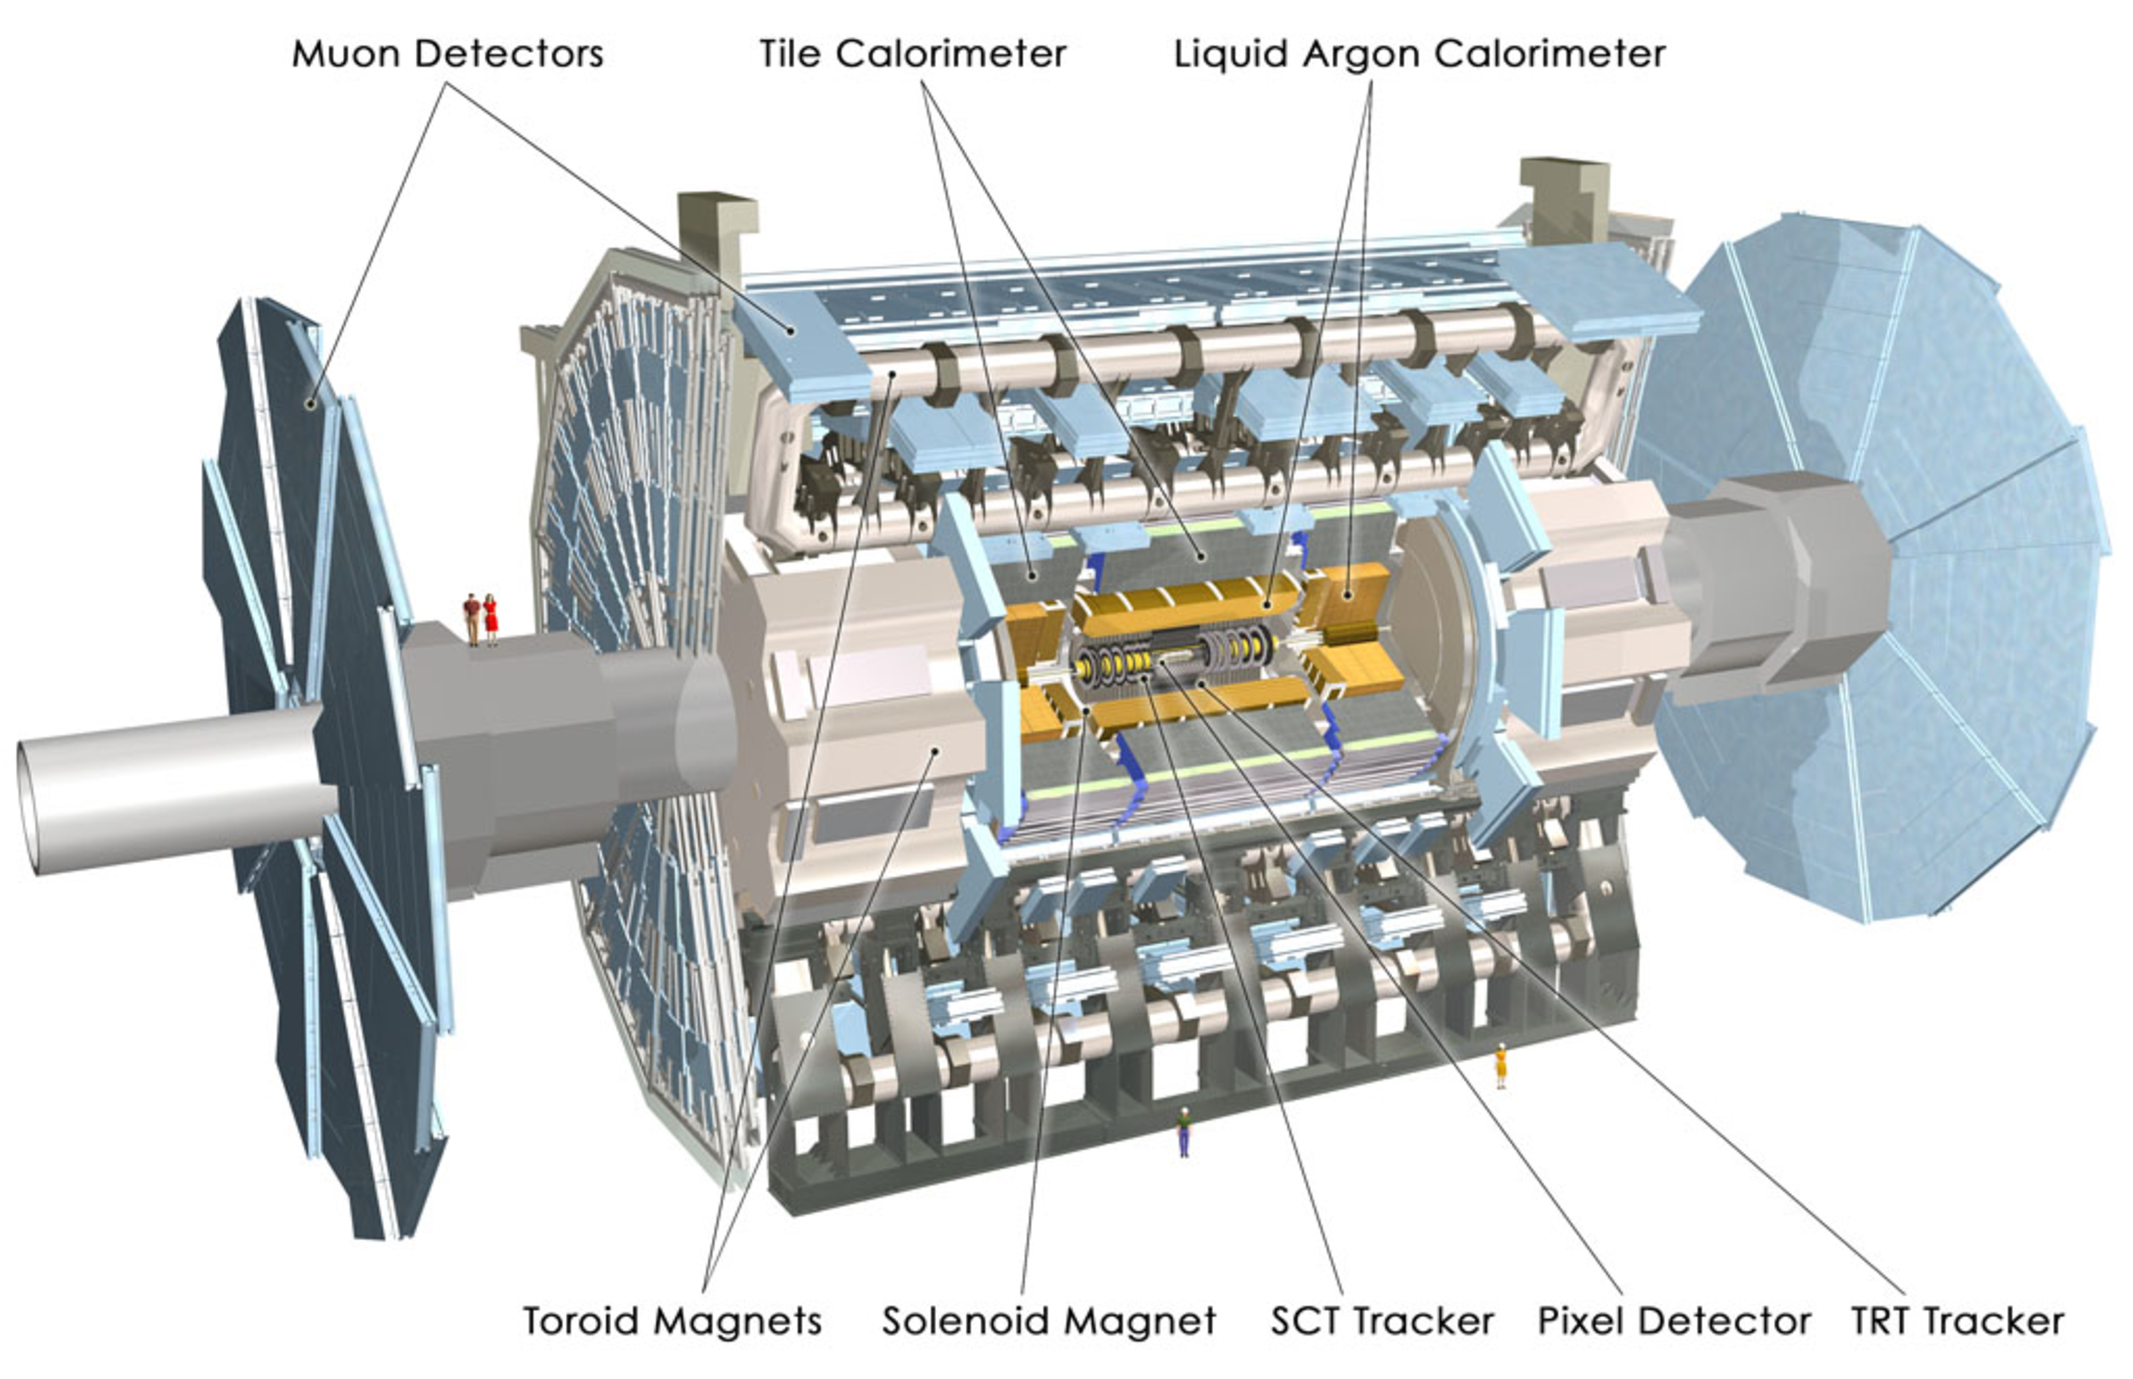
\includegraphics[width=\textwidth]{/Users/caitlinmalone/Documents/Thesis/ATLASDetector/images/AtlasDetectorLabeled.pdf}\label{fig:detector}

%http://www.slac.stanford.edu/econf/C0303241/proc/pres/502.PDF
\section{Trigger}
Although the LHC delivers 20 million bunch crossings per second to the ATLAS detector, the detector does not have the capacity in either storage space or readout bandwidth to record all these collisions.  The trigger has the task of selecting the most interesting 100 or so events per second, which are then fully reconstructed and recorded.  The trigger is a three-layer system, with a first level (L1) implemented solely in hardware, a second level (L2) that reconstructs ``regions of interest'' (RoI's) with special fast algorithms, and an event filter (EF) that reconstructs the full event with offline algorithms.  

L1 reduces the rate from 20 MHz to 70-100 kHz, then L2 reduces an additional factor of 100 to 1 kHz, and about 100 events/second pass the EF.   




